\section{Protokół NMEA 0183}
\label{NMEA}

Niniejszy podrozdział powstał na podstawie źrodeł \cite{inzynierka} oraz \cite{QUECTEL_HW_DESIGN}.\\

Protokół ten stanowi standard komunikacji między urządzeniami elektronicznymi wykorzystywanymi w urządzeniach morskich, zwłaszcza urządzeniami do lokalizacji i nawigacji. Zawiera on specyfikację elektryczną oraz opis ramek (wiadomości) wymienianych między modułami. Powstał w Stanach Zjednoczonych w \textit{\textbf{N}ational \textbf{M}arine \textbf{E}lectronics \textbf{A}ssociation}. Jego najnowsza, czwarta wersja pochodzi z listopada 2008 roku. 
Protokół ten pierwotnie wykorzystywał interfejs RS232, lecz w wersji drugiej dokonano jego zmiany na RS422. Interfejsy te różnią się jedynie poziomami napięć przypisanym logicznym wartościom bitów 0 i 1. 
Oba z nich umożliwiają wysyłanie danych bajt po bajcie. Każdy z nich rozpoczyna się bitem START (stan niski w RS422), który umożliwia odbiornikowi wykrycie początku bajtu i synchronizację. Następnie wysłanych jest kolejno 8 bitów danych, po których przesyłany jest bit parzystości (0 gdy liczba bitów w bajcie danych o wartości 1 jest parzysta lub 1 gdy jest nieparzysta) i na koniec - bit stopu. Przedstawiono to na rysunku \ref{fig:image_nmea_rs422}.

\begin{figure}[H]
	\centering
	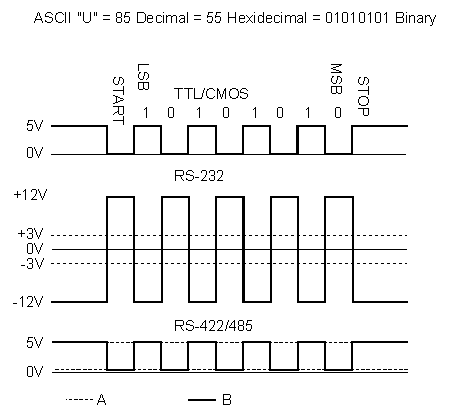
\includegraphics[width=10cm]{img/theory/NMEA/RS232_RS422.png}
	\caption{Poziomy napięć i kolejnośc bitów w interfejsach RS232 i RS422. Źródło: \cite{RS422}}
	\label{fig:image_nmea_rs422}
\end{figure}

Na podstawie tego interfejsu, NMEA nabudowała wyższą warstwę protokołu w postaci wiadomości. Każda wiadomość rozpoczyna się symbolem '\textbf{$\$$}', po którym występuje 2 literowy kod mówiący o type urządzenia (GP - urządzenie GPS, GN - urządzenie GLONASS) i 3 literowy kod definiujący typ przesyłanej wiadomości. Po kodzie występuje przecinek, a następnie lista pól danych oddzielonych przecinkami. W obrębie wiadomości, każde pole ma ściśle określoną funkcję i w razie nie występowania, musi zostać przesłane jako puste. Za ostatnim polem występuje znak '\textbf{*}', po którym znajduje się suma kontrolna, liczona jako funkcja Exclusive Or (XOR) ze wszystkich znaków między '\textbf{$\$$}', a '\textbf{*}' bez ich uwzględnienia. 

Lista zdefiniowanych wiadomości jest bardzo długa, jednak w tabeli \ref{table:table_nmea_messages} zestawiono najpowszechniej wykorzystywane w odbiornikach GPS.

\begin{table}[H]
\centering
\caption{Najczęściej wykorzystywane wiadomości NMEA0183 w odbiornikach GPS.\\ Źródło: \cite{inzynierka}}
\label{table:table_nmea_messages}
\begin{tabular}{| l | l |}
\hline
GGA & Najczęściej wykorzystywane dane związane z ustalaniem pozycji GPS \\  \hline
GGL & Pozycja geograficzna – długość, szerokość \\  \hline
GSA & Informacje o aktywnych satelitach oraz o jakości połączenia \\ 
    & (DOP – \textit{ang.    Dilution of Position}) \\ \hline
GSV & Informacje o satelitach w zasięgu \\ \hline
RMC & Rekomandowane minimum danych GNSS \\ \hline
VTG & Dane o kursie oraz prędkości \\ \hline
ZDA & Wiadomość z aktualnym czasem i datą \\ \hline
\end{tabular}
\end{table}

W niniejszej pracy, aby zrealizować założenia projektu niezbędne było sparsowanie (przeanalizowanie) danych z dwóch wiadomości nadawanych przez moduł GPS: GGA i VTG.
Z wiadomości GGA  wyłoniono informacje o długości i szerokości geograficznej, wskaźnikach półkul, statusie wyznaczenia lokalizacji, jakości odebranego sygnału, liczbie satelitów w zasięgu oraz wysokości nad poziomem morza. Wiadomość VTG została wykorzystana w celu uzyskania informacji o kursie (azymucie) oraz prędkości odbiornika. Ich struktury przedstawiono kolejno w tabelach \ref{table:table_nmea_gga_message} i \ref{table:table_nmea_vtg_message}.

\begin{table}[H]
\centering
\caption{Struktura wiadomości GGA. Źródło: Twórczość własna}
\label{table:table_nmea_gga_message}
\begin{tabular}{| l | l |}
\hline
\textbf{Pole} & \textbf{Opis} \\ \hline
\$ & Symbol początku wiadomości  \\ \hline
GP & Typ urządzenia  \\ \hline
GGA & Typ wiadomości  \\ \hline
130305.743 & Czas UTC w formacie hhmmss.sss \\ \hline
4717.115 & Szerokość geograficzna w formacie ddmm.mmm \\ \hline
N & Wskaźnik półkuli (N - północna, S - południowa) \\ \hline
00833.912 & Długość geograficzna w formacie dddmm.mmm  \\ \hline
E & Wskaźnik półkuli (W - zachodnia, E - wschodnia) \\ \hline
1 & Wskaźnik informujący o statusie wyznaczania pozycji \\ 
 & 0 - pozycja nieustalona \\ 
 & 1 - pozycja ustalona na podstawie sygnału z satelitów \\ 
 & 2 - pozycja ustalona przy pomocy DGPS \\ 
 & 6 - pozycja wyestymowana za pomocą mechanizmu \textit{Dead reckoning} \\ \hline
08 & Liczba satelitów z których odebrano sygnał \\ \hline
0.94 & Wskaźnik jakości sygnału (0.5 - najlepsza, 20 - bardzo niska) \\ \hline
00499 & Wysokość nad poziomem morza \\ \hline
M & Jednostki wysokości (M - metry) \\ \hline
047 & Różnica w wysokości między geoidą (Ziemią), a elipsoidą (przybliżeniem Ziemi) \\ \hline
M & Jednostki wysokości (M - metry) \\ \hline
,, & Dane DGPS (pole puste) \\ \hline
0000 & Numer identyfikacyjny stacji bazowej DGPS \\ \hline
* & Znak końca danych \\ \hline
58 & Suma kontrolna \\ \hline
$<$CR$><$LF$>$ & Znak końca wiadomości \\ \hline
\end{tabular}
\end{table}

\begin{table}[H]
\centering
\caption{Struktura wiadomości VTG. Źródło: Twórczość własna}
\label{table:table_nmea_vtg_message}
\begin{tabular}{| l | l |}
\hline
\textbf{Pole} & \textbf{Opis} \\ \hline
\$ & Symbol początku wiadomości  \\ \hline
GP & Typ urządzenia  \\ \hline
VTG & Typ wiadomości  \\ \hline
227.15 & Kurs (azymut) w stopniach \\ \hline
T & Pole stałe, zawierające symbol T \\ \hline
,, & Kurs magnetyczny (nie zaimplementowany przez producenta) \\ \hline
M & Pole stałe, zawierające symbol M \\ \hline
0.00 & Prędkość \\ \hline
N & Pole stałe opisujące jednostki prędkości (N - węzły, K - kilometry na godzinę) \\ \hline
0.00 & Prędkość \\ \hline
K & Pole stałe opisujące jednostki prędkości (N - węzły, K - kilometry na godzinę) \\ \hline
A & Tryb pozycjonowania \\
  & N - brak pozycji \\
  & A - pozycja na podstawie sygnału z satelitów \\
  & D - pozycja na podstawie DGPS \\ \hline
* & Znak końca danych \\ \hline
3E & Suma kontrolna \\ \hline
$<$CR$><$LF$>$ & Znak końca wiadomości \\ \hline
\end{tabular}
\end{table}

